\documentclass{beamer}
\usepackage[utf8]{inputenc}
\usepackage{graphicx}
\usepackage{verbatim}
\usepackage[absolute,overlay]{textpos} 
\usepackage[francais]{babel}
\usepackage{listings}
\usetheme{Warsaw}

\pgfdeclareimage[width=1in]{fg:logo}{hpc}
\pgfdeclareimage[width=0.68in]{fg:logo2}{p4a} 
\pgfdeclareimage[width=0.8in]{fg:logo3}{smecy}
\pgfdeclareimage[width=0.89in]{fg:logo4}{artemis} 

\renewcommand{\lstlistingname}{Source code}
\lstset{
language=c,
frame=none,
tabsize=2,
captionpos=b
}

\title{Generating SMECY API from annotated sequential code with ROSE compiler}
\author{Vincent \sc Lanore}
\institute{HPC Project Montpellier \\ Encadré par Ronan \textsc{Keryell} \\et Thierry \textsc{Porcher}}

\begin{document}

\begin{frame} 
  \titlepage 
\begin{textblock*}{\textwidth}(.20in,1.7in) 
  \pgfuseimage{fg:logo} 
\end{textblock*}
\begin{textblock*}{\textwidth}(3.95in,1.75in) 
  \pgfuseimage{fg:logo2} 
\end{textblock*}
\begin{textblock*}{\textwidth}(3.89in,2.6in) 
  \pgfuseimage{fg:logo3} 
\end{textblock*} 
\begin{textblock*}{\textwidth}(0.20in,2.5in) 
  \pgfuseimage{fg:logo4} 
\end{textblock*} 
\end{frame} 


\begin{frame}
\frametitle{Plan}
\tableofcontents
\end{frame}

\begin{frame}
\section{Présentation de SME-C}
\subsection{Contexte : Artemis et SMECY}
\frametitle{Contexte : Artemis et SMECY}
\alert{Artemis} (\emph{Advanced Research \& Technology for EMbedded Intelligence and System}) est un projet européen qui regroupe différentes initiatives dans le domaine des \emph{systèmes embarqués}.

\vspace{0.66cm}
\alert{SMECY} (\emph{Smart Multicore Embedded Systems}) fait partie d'Artemis et vise à développer de nouvelles technologies permettant d'utiliser au mieux les \alert{architectures hétérogènes multi-cœurs}. 
\end{frame}

\begin{frame}
\frametitle{Une représentation intermédiaire : SME-C}
SMECY nécessite une \emph{représentation intermédiaire} portable pour faire le lien entre différents outils.
\begin{block}{SME-C}
\alert{SME-C} est langage basé sur le \emph{C99} auquel il ajoute notamment un ensemble de \alert{directives \#pragma} et une API.
\end{block}

\begin{itemize}
	\item API de bas niveau : appel d'accélérateurs matériels
	\item pragmas de haut niveau :
	\begin{itemize}
		\item exécution parallèle
		\item mapping sur accélérateurs matériels
		\item streaming
	\end{itemize}
\end{itemize}
\end{frame}

\begin{frame}
\subsection{Les pragmas SMECY}
\frametitle{Les pragmas SMECY : préambule}
SME-C inclut en particulier les pragmas et l'API d'\alert{OpenMP} pour l'exécution parallèle.

\vspace{0.66cm}
Les pragmas spécifiques à SME-C ont la syntaxe suivante :

\alert{\texttt{\#pragma smecy \emph{clause[[,]clause]... newline}}}
\end{frame}

\defverbatim[colored]\Lstun{%
\begin{lstlisting}
void init(int* array, int size) {
	for (int i=0; i<10; i++)
		array[i]=0;
}

int main() {
	int tab[10][100];
#pragma omp parallel for schedule(static, 1)
	for (int i=0; i<10; i++) {
#pragma smecy map(PE,i) arg(1,out,[10][100],/[i][]) \
                        arg(2,in)
		init(&tab[i][0],100);
	}
	return 0;
}
\end{lstlisting}}

\begin{frame}[fragile]
\frametitle{Les pragmas SMECY : mapping}
\Lstun
\end{frame}

\defverbatim[colored]\Lstdeux{%
\begin{lstlisting}
int main() {
	data_buff data_buffer ;
#pragma smecy stream_loop
	while (1) {
#pragma smecy stream_node(1)
		Produce(data_buffer);
#pragma smecy stream_node(2)
		Consume(data_buffer);
	}
	return 0 ;
}
\end{lstlisting}}

\begin{frame}[fragile]
\frametitle{Les pragmas SMECY : streaming}
\Lstdeux
\end{frame}

\begin{frame}
\section{Conception et implémentation d'un compilateur SME-C}
\subsection{Conception du compilateur}
\frametitle{Idée : réutiliser des outils existants}
Quelques constats :
\begin{itemize}
\item pas question de programmer un compilateur à partir de rien
\item le langage à compiler inclut notamment le C99 et OpenMP ;\\ il existe des compilateurs C99 qui supportent OpenMP. 
\item l'API SMECY a seulement besoin d'être implémentée\\
\end{itemize}
La seule partie réellement nouvelle est la compilation des pragmas SMECY.
\end{frame}

\begin{frame}
\frametitle{Solution : compilation source-à-source}
\og Compilation \fg{} des pragmas SMECY vers l'API SMECY\\avant une compilation classique
\begin{block}{Compilateur source-à-source}
Un \alert{compilateur source-à-source} est un compilateur qui prend un langage de haut niveau en entrée et ressort un langage de haut niveau en sortie.
\end{block}
\vspace{0.35cm}
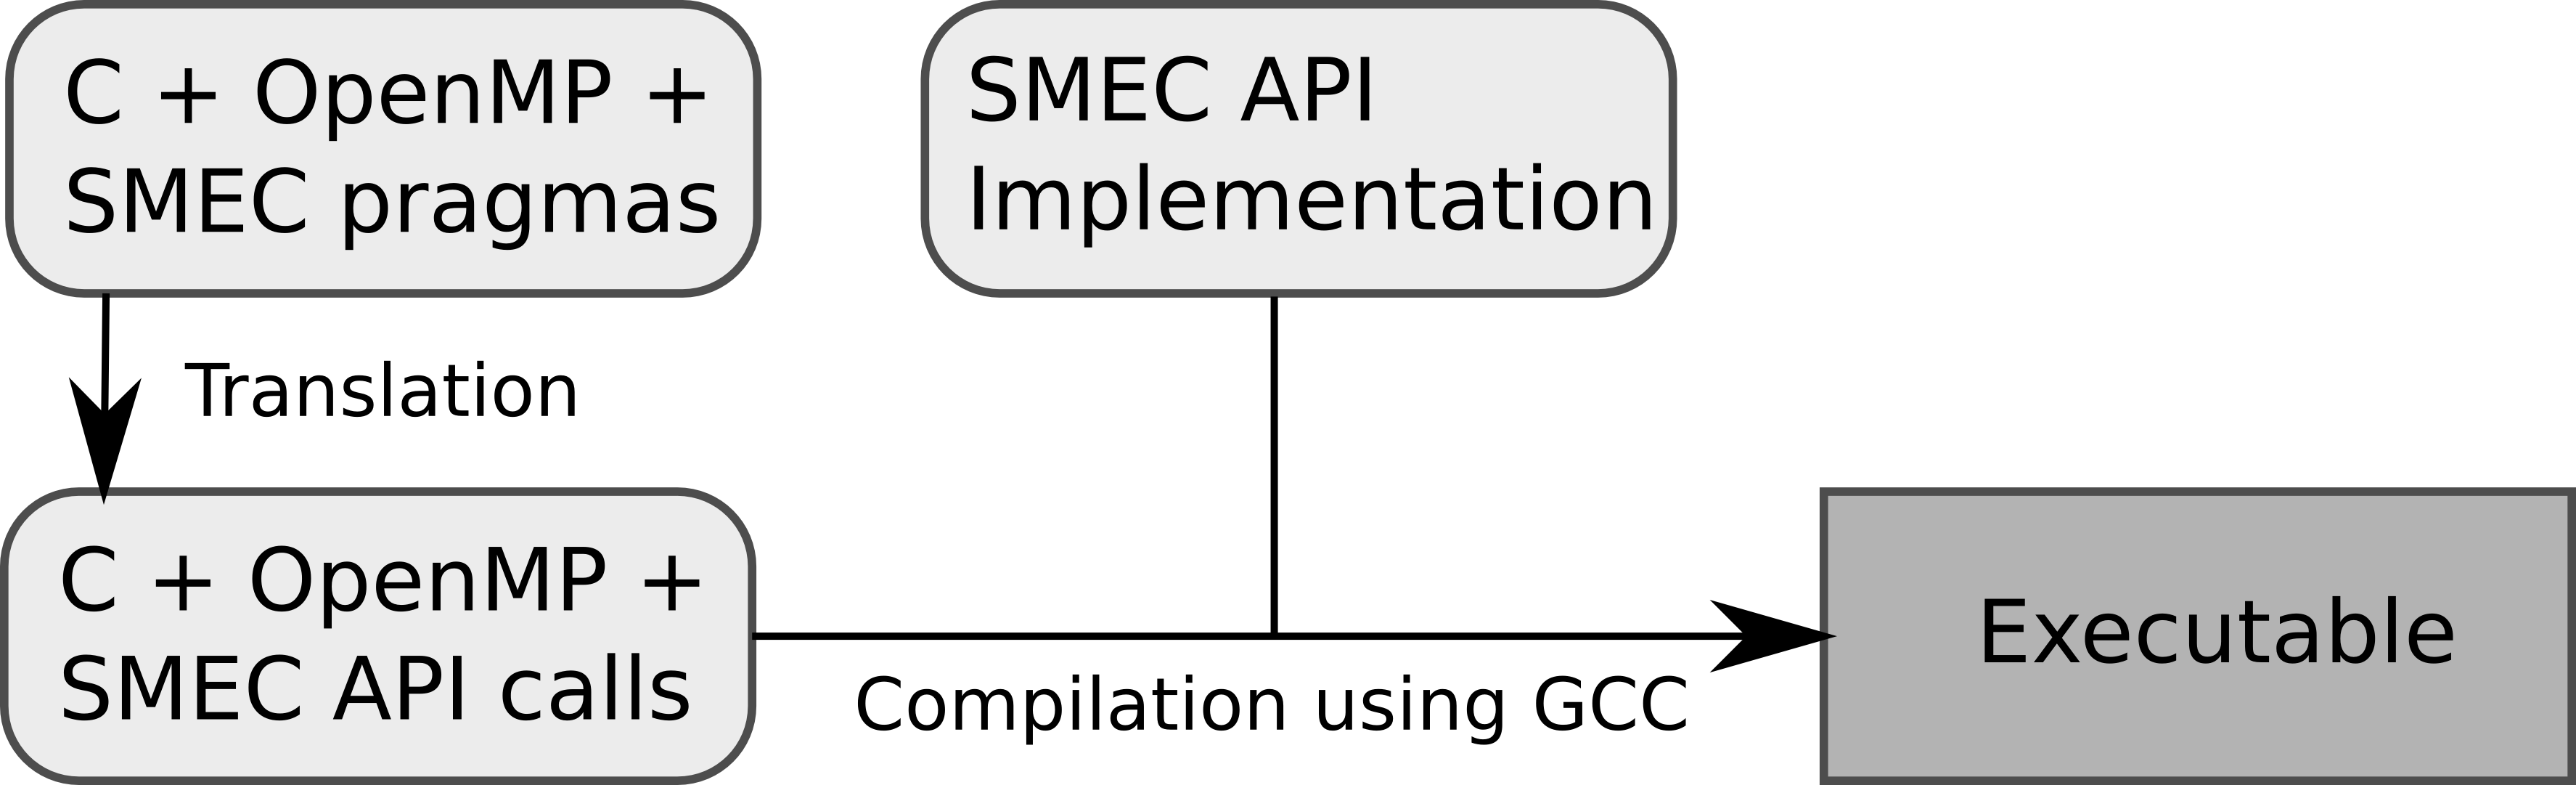
\includegraphics{compiler.png}
\end{frame}

\begin{frame}
\begin{block}{ROSE}
\frametitle{ROSE : un framework pour la compilation source-à-source}
\alert{ROSE} est un framework C++ dédié à la compilation source-à-source.\\
Orienté objet.
Lit et génère du C/C++, FORTRAN...
\end{block} \vspace{0.45cm}
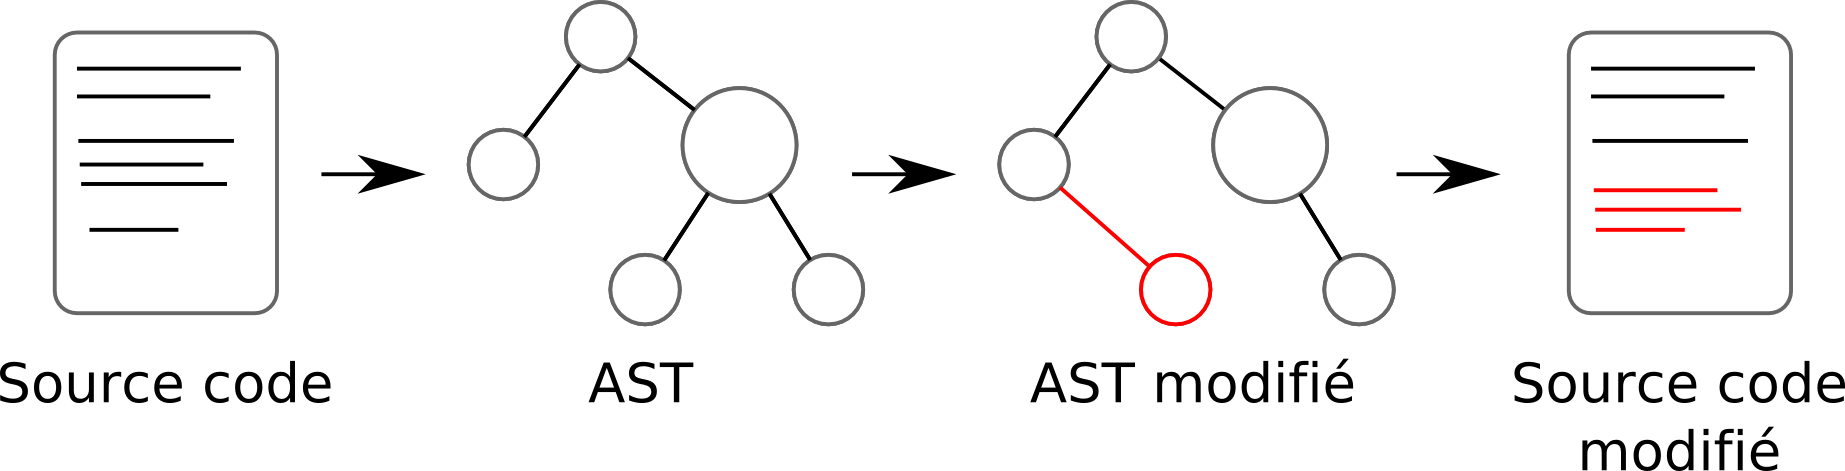
\includegraphics[width=11cm]{rose.png}
\end{frame}

\begin{frame}
\subsection{Implémentation}
\frametitle{Design général du compilateur source-à-source}
ROSE fournit :
\begin{itemize}
\item le front-end,
\item la génération d'AST,
\item les outils pour modifier l'AST,
\item le back-end.
\end{itemize}
Besoin d'un \alert{parseur de directives} pour analyser \\les pragmas SMECY
\end{frame}

\defverbatim[colored]\Lsttrois{%
\begin{lstlisting}[basicstyle=\footnotesize]
#include "smecy.h"

void init(int *array, int size) {
	for (int i=0; i<10; i++)
		array[i]=0;
}

int main() {
	int tab[10][100];
#pragma omp parallel for schedule(static, 1)
	for (int i=0; i<10; i++) {
		SMECY_set(PE,i,init);
		SMECY_send_arg(PE,i,init,2,int,100);
		SMECY_launch(PE,i,init);
		SMECY_get_arg_vector(PE,i,init,
		  1,int,(tab[i] + 0),100);
	}
	return 0;
}
\end{lstlisting}}

\begin{frame}[fragile]
\frametitle{Rappel : mapping}
\Lstun
\end{frame}

\begin{frame}
\frametitle{Mapping : exemple de code transformé}
\Lsttrois
\end{frame}

\begin{frame}
\frametitle{Streaming : utiliser des macros}
SMECY propose une API de bas niveau dédiée au streaming.
Cette API est \alert{complexe à utiliser} dans le cadre de la compilation des pragmas.
\begin{block}{Solution} utiliser des \alert{macros C} pour encapsuler les appels à l'API.\\
On y gagne en clarté, simplicité du compilateur et en indépendance avec l'API.
\end{block}
\end{frame}

\defverbatim[colored]\Lstquatre{%
\begin{lstlisting}[basicstyle=\scriptsize]
#include "p4a_macros.h" 

struct __buffer_type_0 {
	int data_buffer;
};

void __Node_0_0() {
	__buffer_type_0* struct_buffer;
	p4a_stream_get_init_buf(0);
	while(1){
		Produce(struct_buffer -> data_buffer);
		p4a_stream_put_data(0);
	}
}

void __Node_0_1() {
	__buffer_type_0 *struct_buffer;
	while(1){
		p4a_stream_get_data(0);
		Consume(struct_buffer -> data_buffer);
	}
}

int main() {
	data_buff data_buffer ;
	p4a_init_stream(0);
	p4a_launch_stream(0,0);
	p4a_launch_stream(0,1);
	pause();
	return 0;
}
\end{lstlisting}}

\begin{frame}[fragile]
\frametitle{Rappel : streaming}
\Lstdeux
\end{frame}

\begin{frame}
\frametitle{Streaming : exemple de code transformé avec macros (1)}
\Lstquatre
\end{frame}

\defverbatim[colored]\Lstcinq{%
\begin{lstlisting}
int main() {
	data_buff data_buffer ;
	p4a_init_stream(0);
	p4a_launch_stream(0,0);
	p4a_launch_stream(0,1);
	pause();
	return 0;
}
\end{lstlisting}}

\begin{frame}
\frametitle{Streaming : exemple de code transformé avec macros (2)}
\Lstcinq
\end{frame}

\begin{frame}
\frametitle{Tests : pas simple sans implémentation de l'API}
La translation source-à-source a pu être testée et fonctionne.\\ On ne peut pas tester le compilateur complet car il n'y a pas encore d'\alert{implémentation de l'API}.\\ \vspace{0.66cm}Implémentation d'une \og API jouet \fg{}. Tests concluants.\\Implémentation spécifique d'une  \og API jouet \fg{} utilisant OpenMP pour simuler un accélérateur matériel.
\end{frame}

\begin{frame}
\frametitle{Conclusions}
\begin{itemize}
	\item Travail en entreprise, intégration à un projet ;
	\item partie technique en autonomie ;
	\item programme final fonctionnel.
\end{itemize}
\end{frame}

\begin{frame}
Merci de votre attention.\\ \vspace{0.66cm} Y a-t-il des questions ?
\end{frame}
\end{document}